\chapter{Installation}

\section{Prerequisites}

\begin{itemize}
	\item This package aims at automating GSAS, therefore, a running GSAS is required. To test this, at the command line from which you wish to run this (mouse junkies - this will NOT be your cup of tea� but maybe we can pull you into the great land of command lines) change into a folder with GSAS data and try to plot it in rawplot by typing in rawplot. If this fails with a file not found error, GSAS is either not installed or not in the search path. If it plots, but doesn't have text around the graph, the PGPLOT\_FONT variable is not set. Another missing bit could be the GSAS variable, in which case GSAS wouldn't know where to look for the scattering length etc. All this is documented in the README file coming with GSAS, but who reads those these days...
	\item The 2nd prerequisite is a working understanding of GSAS by the user. If you don't know what GSAS does and how it works, this here will be of little help, it might be even dangerous... We strongly suggest you work at least through the excellent tutorials that come with GSAS to get an idea what GSAS does.
\end{itemize}

\section{Linux or Windows?}

We found that the same stuff runs a lot (factor 2 up to 5) faster when a given system runs under Linux. Using the bash shell provides much easier access for fast development of tools like this than the windows shell.

\section{Linux/Mac/Unix Installation}

\begin{itemize}
\item Copy the scripts into an appropriate folder and add it to the path. Done.
ok, maybe not completely. Make sure you have LaTex installed (punch in ``latex'' at a command prompt, it should come up with a LaTeX prompt). If you want to plot the results of a multi-run analysis using gsas\_plot\_overview, make sure you have gnuplot installed.
\end{itemize}

\section{Windows Installation}

\begin{itemize}
\item Copy the scripts into an appropriate folder, e.g. c:$\backslash$gsas\_language 
\item Since we need a bash shell, install the cygwin package from (www.cygwin.com).  Download the setup executable and store it in the same folder where you will install cygwin (e.g.c:$\backslash$ cygwin). That way it can be used for future additions and updates. Provide your internet options. If you are working at a government lab, choose a cygwin site at another government lab (.gov) since they are connected with a high-speed backbone. Once you see the ``select packages'' screen (see screenshot below), click on the ``View'' button in the top right corner until you see the ``Full'' view. Besides the basic cygwin, select to install also gnuplot.  Make sure to follow the UNIX end-of-line convention, if in doubt (getting weird error messages when running the gsas scripts such as ``unexpected end of file'' or so), run ``dos2unix'' on your script from the command line.
\begin{figure}[h]
\centering
	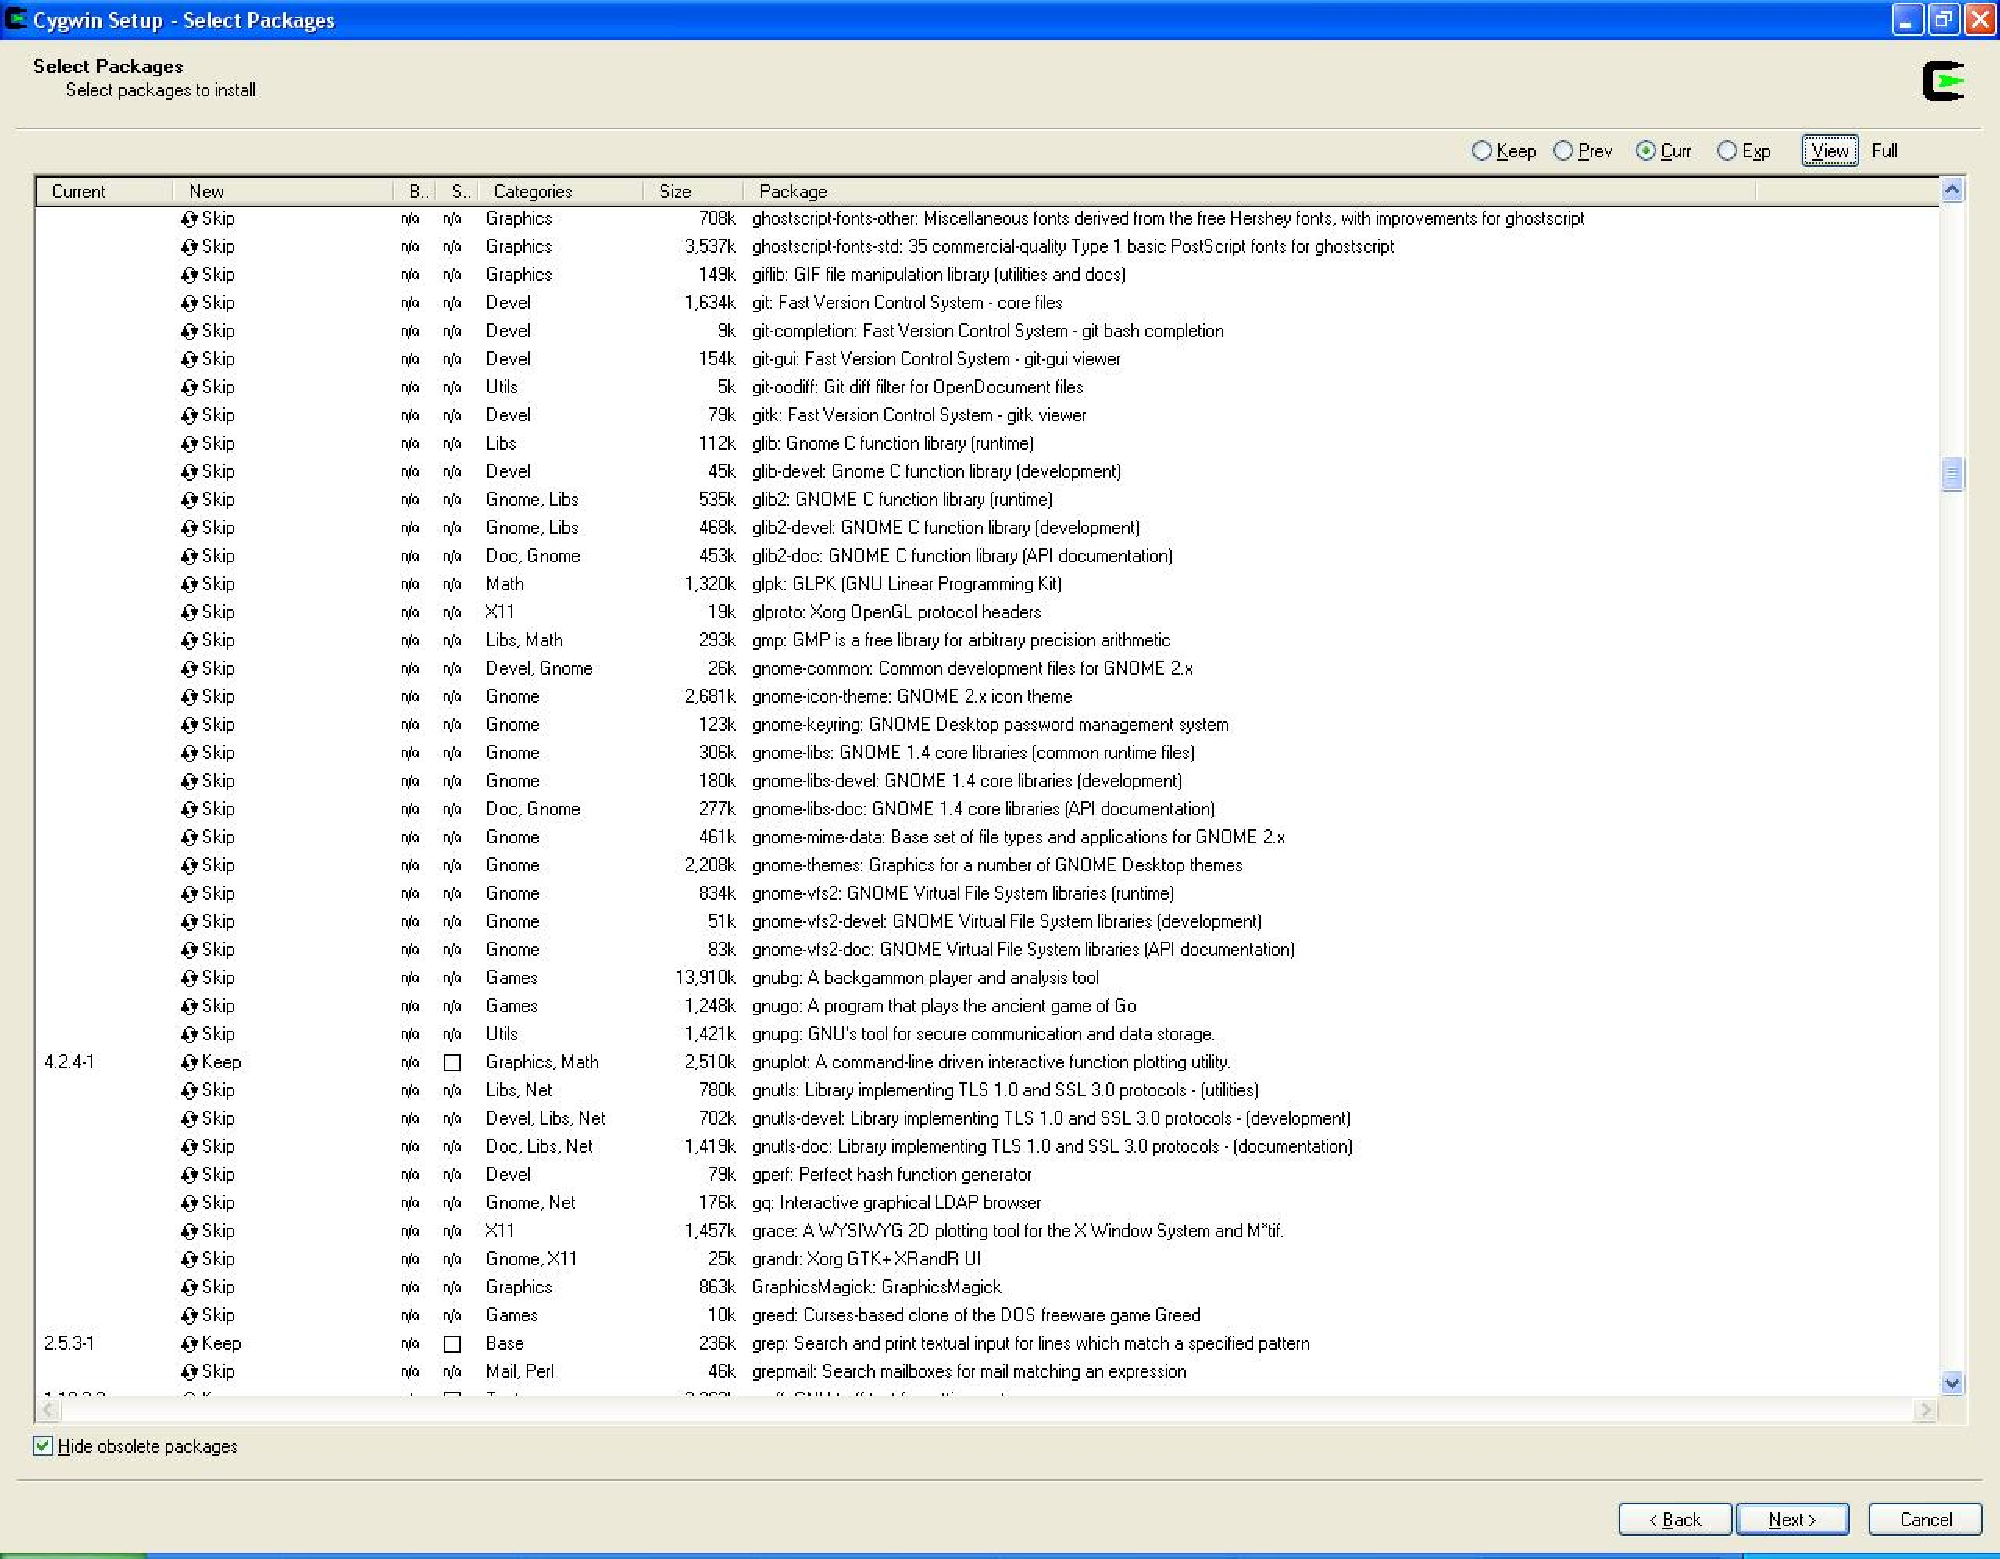
\includegraphics[width=12cm]{Screenshot1.pdf}
\caption{Selecting packages during Cygwin installation}
\label{fig:Screenshot1}
\end{figure}

\item Get the GSAS scripts (ZIP files named something like
``gsas\_language.zip'' from Sven -- or steal it from the HIPPO data room computer. Unzip the contents into a folder of your choice.
 Add the folder name to the search path (Control Panel -- System -- Advanced
-- Environment Variables -- PATH)
\item Install LaTex (go to miktex.org to download the basic installation for a Windows system).
\item You may have to install the LaTeX package fullpage manually if your firewall does not allow LaTeX to install it on the fly. If you are using Miktex (Basic MiKtex 2.7), install it into a subfolder of your Miktex installation and refresh the Filename database in the Miktex options.
\end{itemize}

